\chapter{API}
\label{sec:module.API}

Unsere AITools API dient als Grundbaustein aller AI Komponenten und entkapselt die Interfaces zu unseren AI Modulen und bietet den AI Modulen sowie dem Ants Package die Basisklassen an, welche �berall verwendet werden. (siehe Abbildung \ref{fig:modulesOverview}) Der Inhalt ist wie folgt:

\section{Entities}
\label{sec:mocule.API.Entities}

Das Package Entites beinhaltet alle Klassen die im von den Such- und Strategiealgorithmen sowie von Bot verwendet werden.

\begin{figure}[H]
\centering
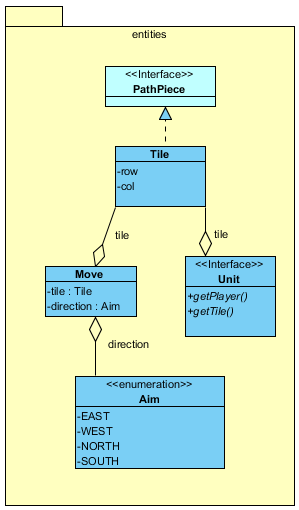
\includegraphics[height=90mm]{91_bilder/apiEntities}
\caption{Entities}
\label{fig:apiEntities}
\end{figure}

\begin{itemize}
\item
\textbf{Aim}: Richtungangabe zum Beschreiben einer Bewegung der Ameise
\item
\textbf{Tile}: Repr�sentiert eine Zelle auf dem Spielfeld, welche mit Row (Zeile) und Column (Spalte) beschrieben ist.
\item
\textbf{Move}: Diese Klasse beschreibt einen Spielzug mit den Eigenschaften Tile, von wo aus der Zug statt findet, und Aim, in welche Richtung der Zug ausgef�hrt wird.
\item
\textbf{Unit}: Unit besteht aus Tile und Spieler und definiert eine Einheit eines Spielers auf der Karte.
\end{itemize}

\section{Map}
\label{sec:mocule.API.Map}

Im Map-Package wird definiert welche Eigenschaften und Funktionen die Spielkarte hat und von welchem Typ (TileMap) sie ist.

\begin{figure}[H]
\centering
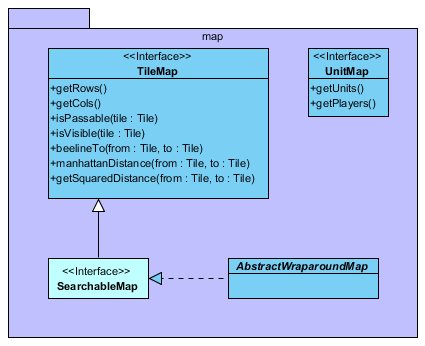
\includegraphics[width=0.7\textwidth]{91_bilder/apiMap}
\caption{Map API}
\label{fig:apiMap}
\end{figure}

\begin{itemize}
\item
\textbf{TileMap}:  Dieses Interface definiert, welche Methoden eine auf Tiles aufbauende Spielkarte anbieten muss. Dazu geh�ren die Masse der Karte, die Gel�ndebeschaffenheit, also ob eine Zelle f�r den Spieler sichtbar und passierbar ist, sowie Distanz-Messfunktion wie ManhattanDistance, Luftlinie, quadrierte Distanz.
\item
\textbf{AbstractWraparoundMap}: Implementiert das Interface SearchableUnitMap (siehe: Kapitel \titleref{sec:module.Suchalgorithmen}). Hier sind alle Methoden implementiert, welche die Karte anbieten muss, damit sie mit den Suchalgorihmen verwendet werden kann. Zudem sind die vordefinierten Methoden aus TileMap implementiert.
\item
\textbf{WorldType}: WorldType ist ein Enum und definiert die Art der Karte. Der Typ \textit{Globus} hat keine Kartenr�nder, ist also ringsum begehbar. Von diesem Typ ist auch die AbstractWraparoundMap Klasse, welche die Basiskarte unserer World-Karte\footnote{Die Klasse World ist im Code unter ants.state.World eingegliedert.} ist. Folglich sind auch die Karten  der Ants Challenge 'WrapAround'-Karten. Der zweite Enumtyp ist \textit{Pizza} und definiert eine Welt so wie man sich unsere Erde vor 500 Jahren noch vorstellte, eine Scheibe mit R�ndern, welche die Welt begrenzen. Dieser zweite Typ wurde provisorisch erstellt. Falls unsere API eine Weiterverwendung findet, kann dieser Typ zus�tzlich implementiert werden.
\end{itemize}


\section{Search}
\label{sec:mocule.API.Search}

Search beinhaltet alle Basisklassen und -interfaces der Suche.

\begin{figure}[H]
\centering
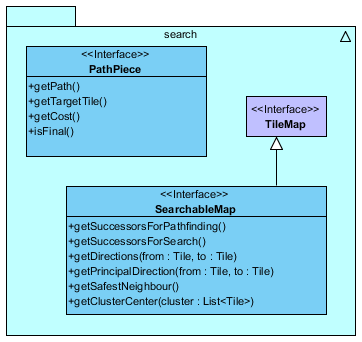
\includegraphics[width=0.6\textwidth]{91_bilder/apiSearch}
\caption{Search API}
\label{fig:apiSearch}
\end{figure}

\begin{itemize}
\item
\textbf{PathPiece}: Das PathPiece ist ein Interface f�r Strukturen, die als Suchknoten in der Pfadsuche verwendet werden k�nnen. Implementierende Klassen sind Edge (rep�sentiert eine Kante in einem Cluster) und Tile. Erweiterungen dieser Klassen sind DirectedEdge (gerichtete Kanten) und Vertex (ein Knoten mit anliegenden Kanten).
\item
\textbf{SearchableMap}: Das Interface SearchableMap erweitert das Interface TileMap. Es beschreibt die Methoden zur Pfadsuche, wie getSuccessors(), getCost(), oder getPath().
\end{itemize}

\section{Strategy}
\label{sec:mocule.API.Strategy}

In diesem Package befinden sich die Karteninterfaces, welche f�r das Anwenden von Strategie und Taktikalgorithmen grundlegend sind.

\begin{figure}[H]
\centering
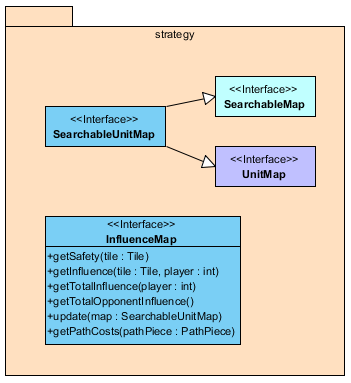
\includegraphics[width=0.6\textwidth]{91_bilder/apiStrategy}
\caption{Strategy API}
\label{fig:apiStrategy}
\end{figure}

\begin{itemize}
\item
\textbf{UnitMap}: UnitMap ist auch ein Interface welches auf TileMap aufbaut und zus�tzlich die Methoden definiert um Einheiten und Spieler zu verwalten.
\item
\textbf{SearchableUnitMap}: Dieses Interface dient ausschliesslich zur Zusammenf�hrung der beiden Interfaces UnitMap und SearchableMap.
\end{itemize}